\section{Convolutional Neural Networks}

    A convolutional neural network (also known as CNN) is a deep neural network inspired in the behavior of biological systems through artificial neurons with learnable weights and biases for image recognition tasks.
    D.H Hubel and T.N Wiesel discovered that the visual cortex consists of receptive fields that detect light in overlapping subregions.
    It is the entry point of modeling CNNs \cite{hubel1968receptive}.
    Every neuron responds to stimuli in a restricted region, as in visual cortex of the human brain, and that the overlapping regions of the neurons together cover the entire visual area.

    \begin{figure}
    \centerline{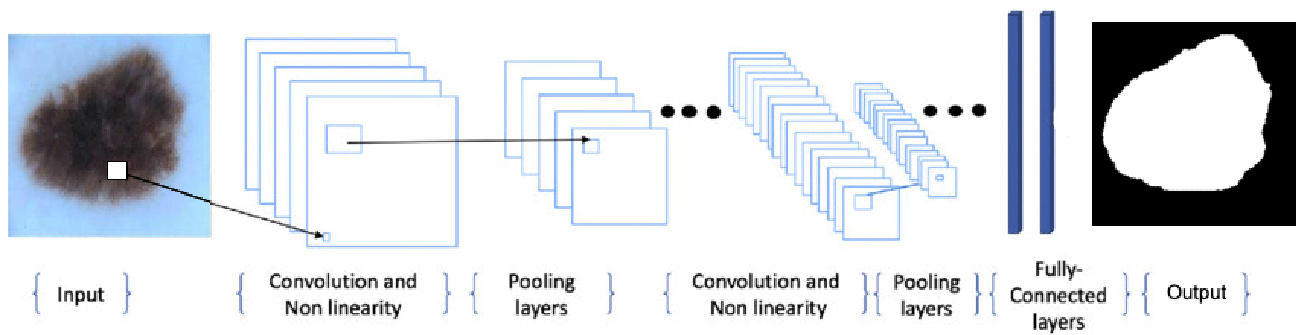
\includegraphics[width=1\columnwidth]{03-neural-networks-in-tumor-detection/figures/cnn-architecture-image-classification.png}}
    \caption{A CNN architecture for skin lesion classification}
    \label{figure:sample-cnn-architecture-skin-lesion-classification}
\end{figure}

    A CNN mainly consist of different types of layers as it can be seen in Figure~\ref{figure:sample-cnn-architecture-skin-lesion-classification} including input, convolutional, non-linearity, pooling, and fully connected layers.

    \begin{itemize}

        \item \textbf{Input layer} contains input images as a matrix of the raw pixel values.

        \item \textbf{Convolutional layer} is used to extract features of the input data.
            Each neuron has a local receptive field which means it is not fully connected, but connected to some section of the input to provide abstractions of small sections of the input data.
            Convolution layers calculate a dot product between the receptive field and the filter by performing convolution.
            The result of this convolution is a single integer which will be used as the input of the next layer.

            The filter is slided over the next receptive fields of the input image repeatedly until there is no unconvolved receptive field left.

        \item \textbf{Non-linearity layer} consists of an activation function, which applies an elementwise activation by thresholding at zero, creates and activation map with taking the output of the convolutional layer in CNNs.

        \item \textbf{Pooling layer} apply a spatial downsampling along the output volume.
            Pooling layers are commony used to reduce the computational requirements of the neural networks progressively and minimize the overfitting \cite{Layersof6online}.

        \item \textbf{Fully connected layer} mainly computes the class scores based on the training dataset.
            They connect the neurons in layers to each other.
            The last fully connected layer classifies the generated features with the help of an activation function.

    \end{itemize}


